\section{Clase 2. Tangram}
\textbf{12/02/2025}
\section{Elaborando las piezas}

Cada pieza durante la clase fue elaborada por medio de origami y los materiales necesarios fueron solo 4 cuadrados de papel del mismo tamaño. El tangram consta de 7 figuras y su realización se detalla a continuación:

\begin{itemize}
    
    \item Triángulos grandes
    \begin{enumerate}

        \item  Se necesitan 2 cuadrados grandes de papel
        \item Toma un cuadrado grande.  
        \item Dóblalo por la mitad de forma vertical y luego horizontal (lleva el lado derecho hacia la izquierda y el inferior hacia arriba), de modo que el papel quede dividido en cuatro secciones iguales.  
        \item Con cada uno de los cuatro cuadrados, lleva la esquina hacia el centro, doblando en diagonal. Puedes comenzar por la esquina superior, luego la izquierda y, finalmente, la inferior.  
        \item Desdobla solo una de las esquinas y utiliza el pliegue existente para volver a doblar el papel por la mitad verticalmente.  
        \item Dobla nuevamente el papel por la mitad, llevando la esquina inferior hacia arriba.  
        \item Abre la primera capa para formar un hueco triangular y mete la esquina restante en él, asegurando la figura en forma de triángulo.  
        \item Realiza el mismo proceso con otro cuadrado grande para obtener el segundo triángulo grande.
        
    \end{enumerate}

    \item Rombo
    \begin{enumerate}

        \item Se necesita 1 cuadrado grande de papel
        \item Dobla el cuadrado por la mitad, llevando el lado inferior hacia arriba para dividirlo en dos rectángulos.  
        \item Desdóblalo y, en cada uno de los rectángulos, dobla horizontalmente llevando el borde hacia el centro.  
        \item Manteniendo el papel doblado, en el lado derecho, dobla la esquina formando un ángulo de 45 grados.  
        \item Utiliza este pliegue como referencia para hacer un nuevo pliegue vertical, llevando el papel de forma precisa. Repite el mismo procedimiento en la parte inferior.  
        \item Desdobla y abre el papel; luego invierte la esquina utilizando los pliegues recién realizados, empujando el centro y revirtiendo la diagonal derecha.  
        \item Cierra el papel y aplánalo.  
        \item Con el último pliegue como guía, realiza un nuevo pliegue vertical.  
        \item Dobla la esquina superior, desdóblala, ábrela e inviértela, y luego haz lo mismo con la esquina superior izquierda.  
        \item Abre el lado derecho, introduce el papel restante en su interior y cierra con precisión. Para asegurar la pieza, coloca la última esquina dentro del espacio de la primera capa; para facilitarlo, dóblala diagonalmente, desdóblala y luego insértala.  
        \item El rombo está listo.
        
    \end{enumerate}
    
    \item Cuadrado
    \begin{enumerate}

        \item Se necesita 1 cuadrado de papel del mismo tamaño que los anteriores
        \item Dobla el cuadrado por la mitad verticalmente (lado derecho a izquierda) y luego horizontalmente (lado inferior hacia arriba).  
        \item Dobla únicamente las esquinas superiores hacia el centro, lo que formará un rectángulo en la parte superior.  
        \item Dobla el rectángulo por la mitad y lleva el lado derecho hacia el centro.  
        \item Usando un pliegue existente, dobla el lado inferior hacia arriba; de esta forma se formará un triángulo en la parte superior.  
        \item Dobla el triángulo hacia abajo siguiendo el borde, desdóblalo y coloca la esquina resultante dentro de la primera capa.  
        \item Utiliza el pliegue sobrante como guía para reforzar el cierre.  
        \item Voltea el papel; en el reverso se formará un pequeño cuadrado con un hueco.  
        \item Mete el papel restante en el hueco. Para facilitar el proceso, dobla ligeramente las esquinas antes de insertarlas. El cuadrado está listo.
    \end{enumerate}
    
    \item Triángulo mediano
    \begin{enumerate}
        
        \item Se necesita 1 rectángulo de papel (con dimensiones equivalentes a la mitad del tamaño de los cuadrados grandes)
        \item Dobla el rectángulo de papel para formar dos cuadrados, llevando el lado derecho hacia la izquierda.  
        \item Desdóblalo y toma el cuadrado derecho; dóblalo en diagonal, llevando la parte superior hacia la línea central.  
        \item En el cuadrado izquierdo, dobla la parte inferior hacia la línea central, formando dos triángulos.  
        \item Dobla el triángulo de la izquierda por la mitad, llevando la esquina hacia el lado inferior y alineando el borde con la línea central.  
        \item Dobla esta pieza sobre el otro triángulo y mete la esquina restante en el hueco resultante para asegurar la figura.  
        
    \end{enumerate}
    
    \item Triángulos pequeños
    \begin{enumerate}
        
        \item Se necesitan 2 cuadrados de papel (cada uno con tamaño equivalente a un cuarto del cuadrado grande)
        \item Dobla el cuadrado por la mitad de forma vertical y luego horizontalmente.  
        \item Dobla las cuatro esquinas hacia el centro del cuadrado.  
        \item Desdobla únicamente una de las esquinas.  
        \item Dobla el papel por la mitad utilizando el pliegue existente y luego vuelve a doblarlo, llevando la esquina hacia arriba.  
        \item Mete la esquina restante dentro de la primera capa para bloquear la figura en forma de triángulo.  
        \item Realiza el mismo proceso con el otro cuadrado para obtener el segundo triángulo pequeño.
        
    \end{enumerate}

    \section{Actividad}

Durante la clase después de realizar cada figura, debíamos formar las siguientes figuras:
            
                
    \hbox{
            \begin{tabular}{c c c c c }
                \hline
                Cuadrado & Rectángulo & Triángulo equilatero & Triángulo rectángulo & Rombo \\\\ \hline
                \\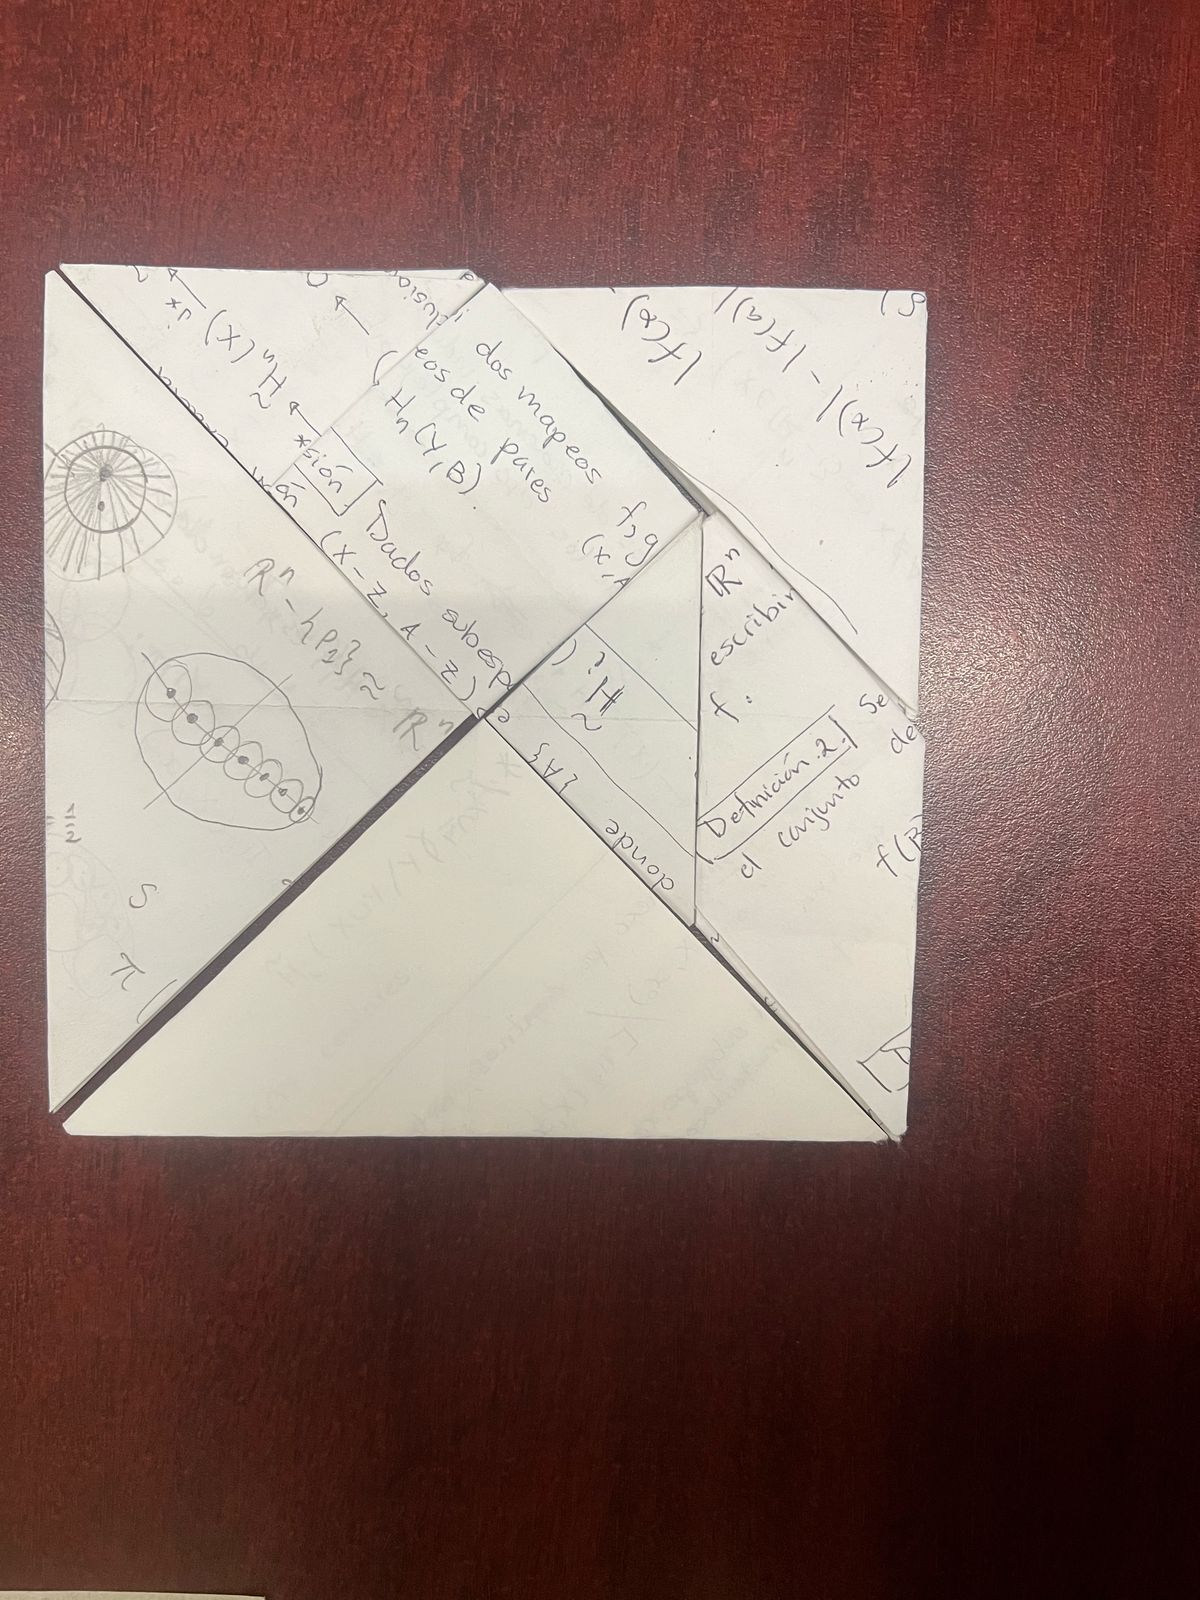
\includegraphics[scale=0.05]{clase2/cuadrado.jpeg} & 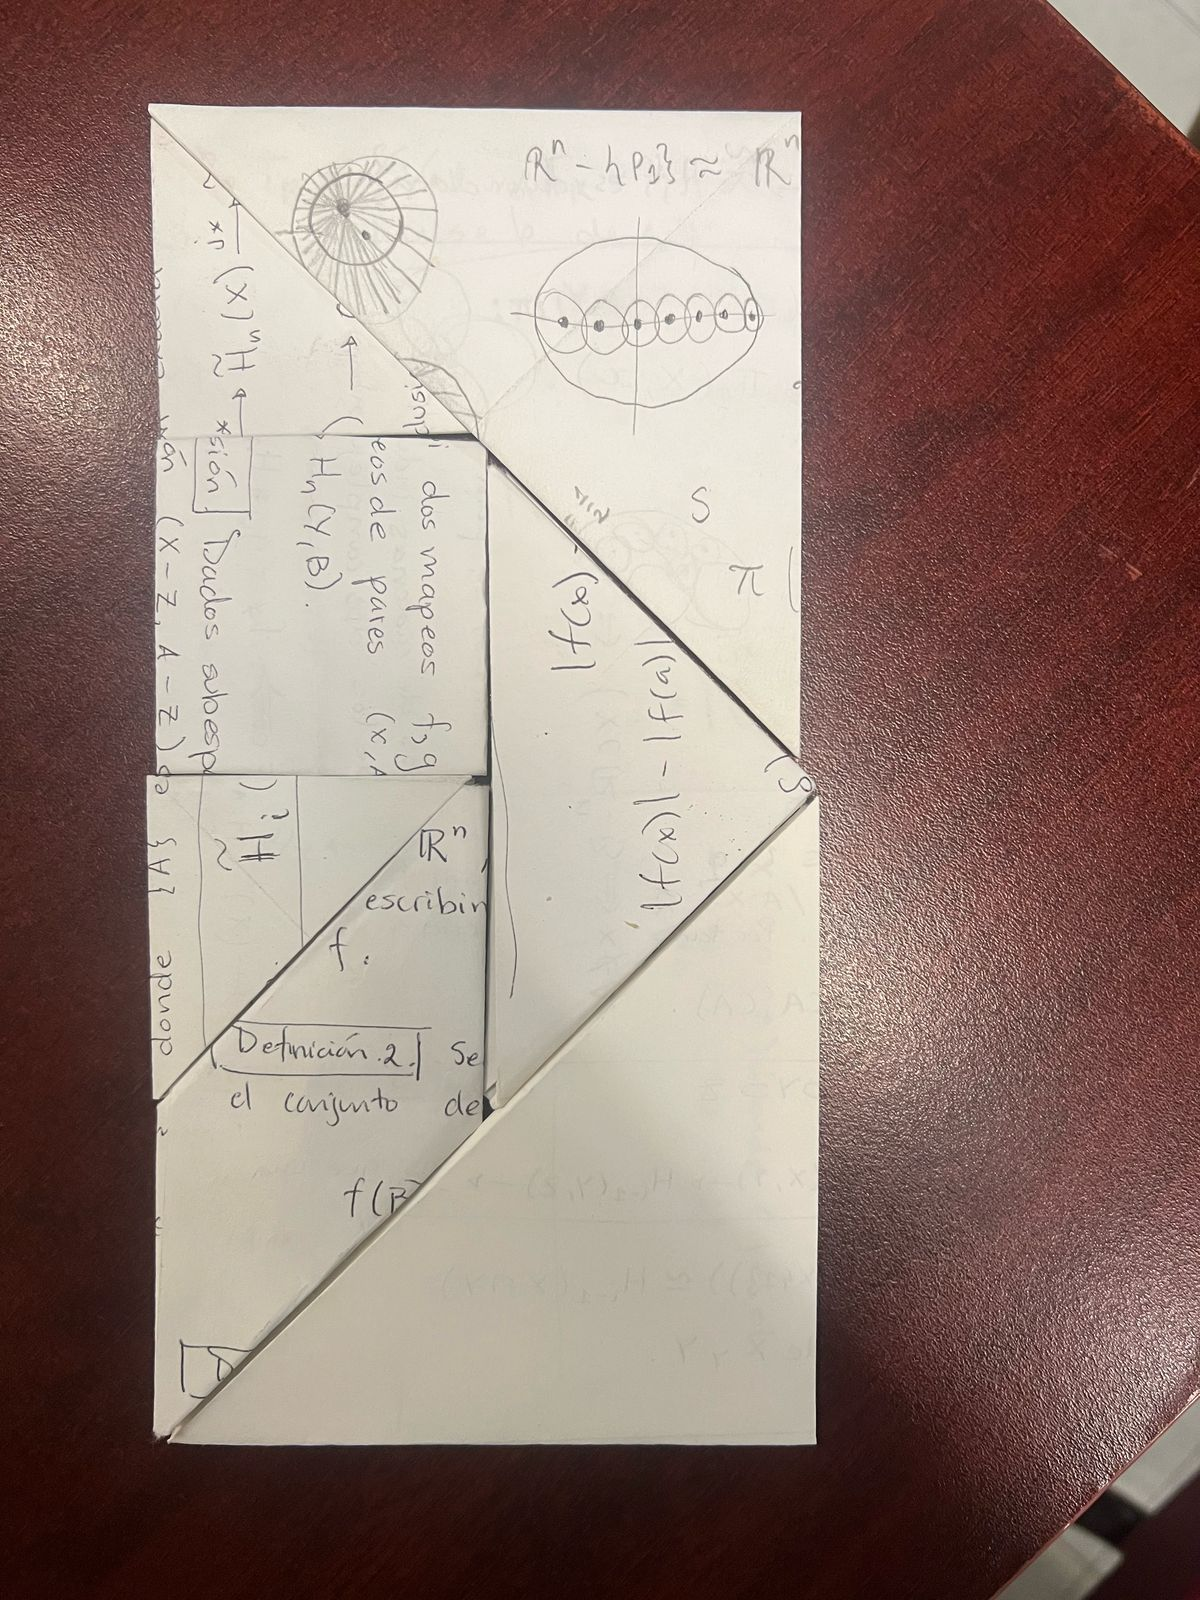
\includegraphics[scale=0.05]{clase2/rectangulo.jpeg} & &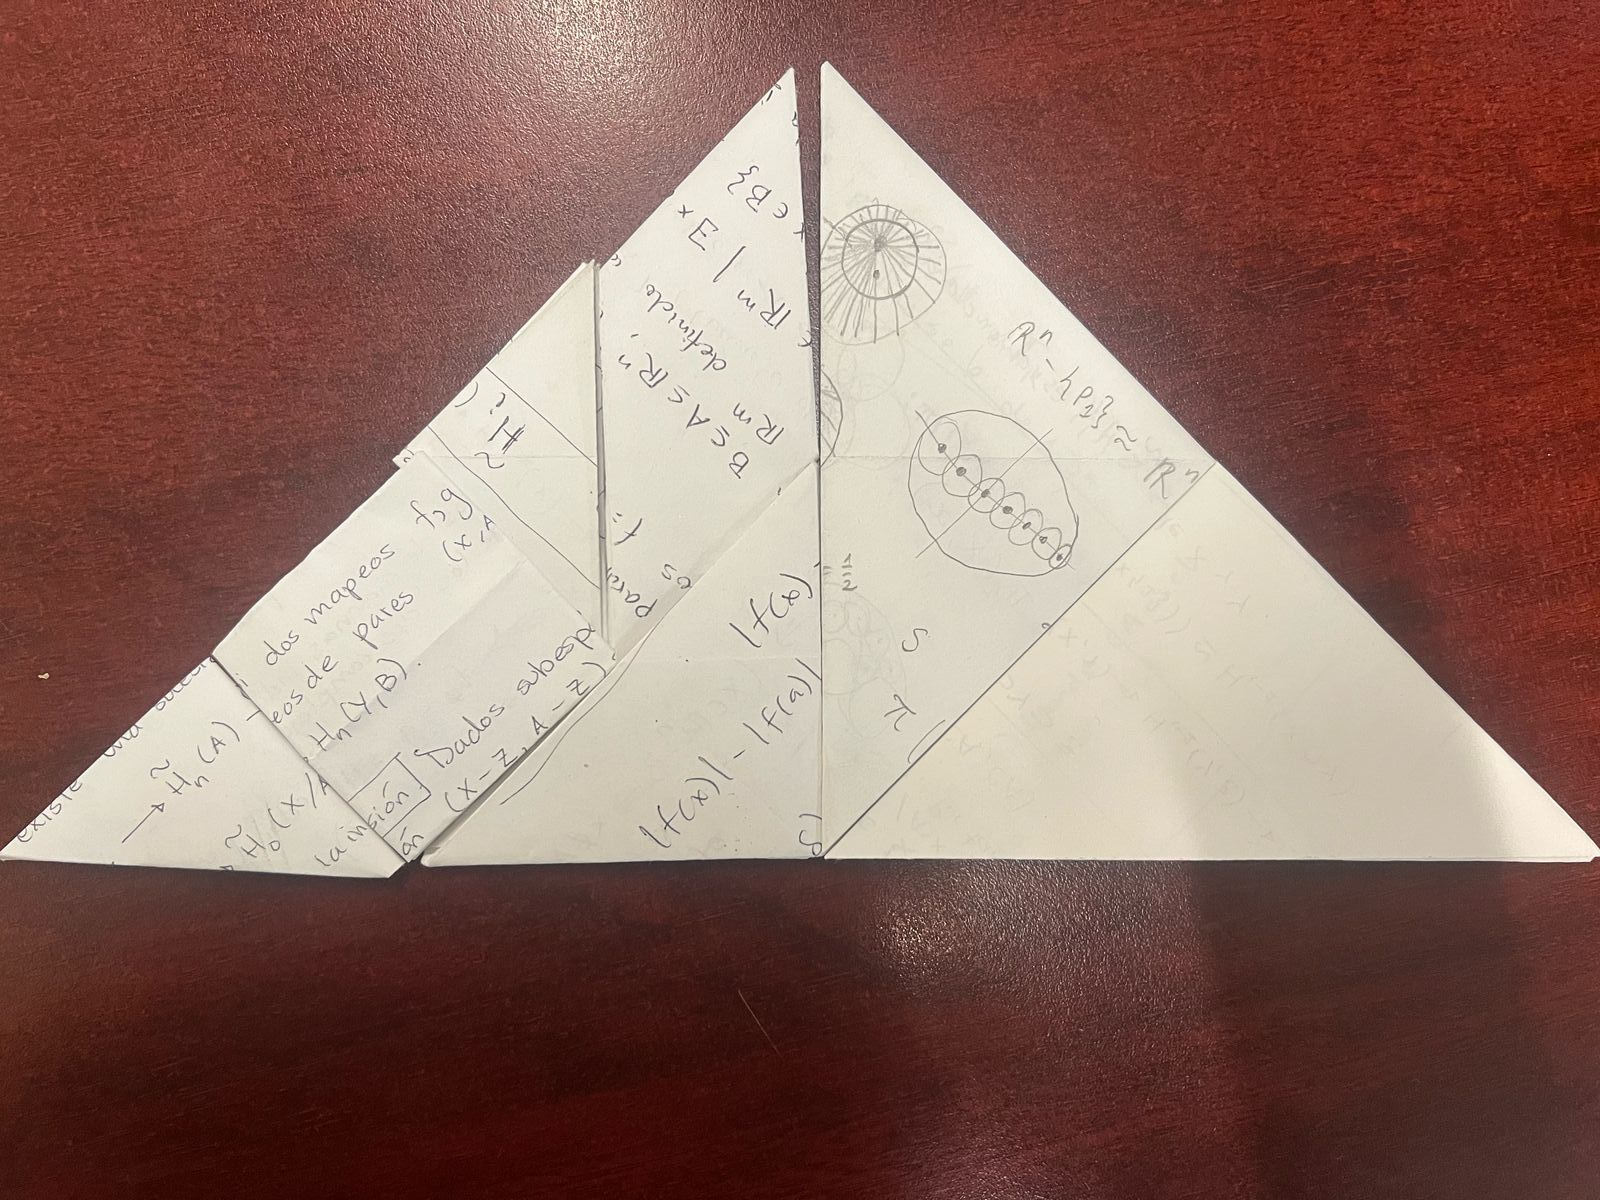
\includegraphics[scale=0.05]{clase2/equilatero.jpeg} & 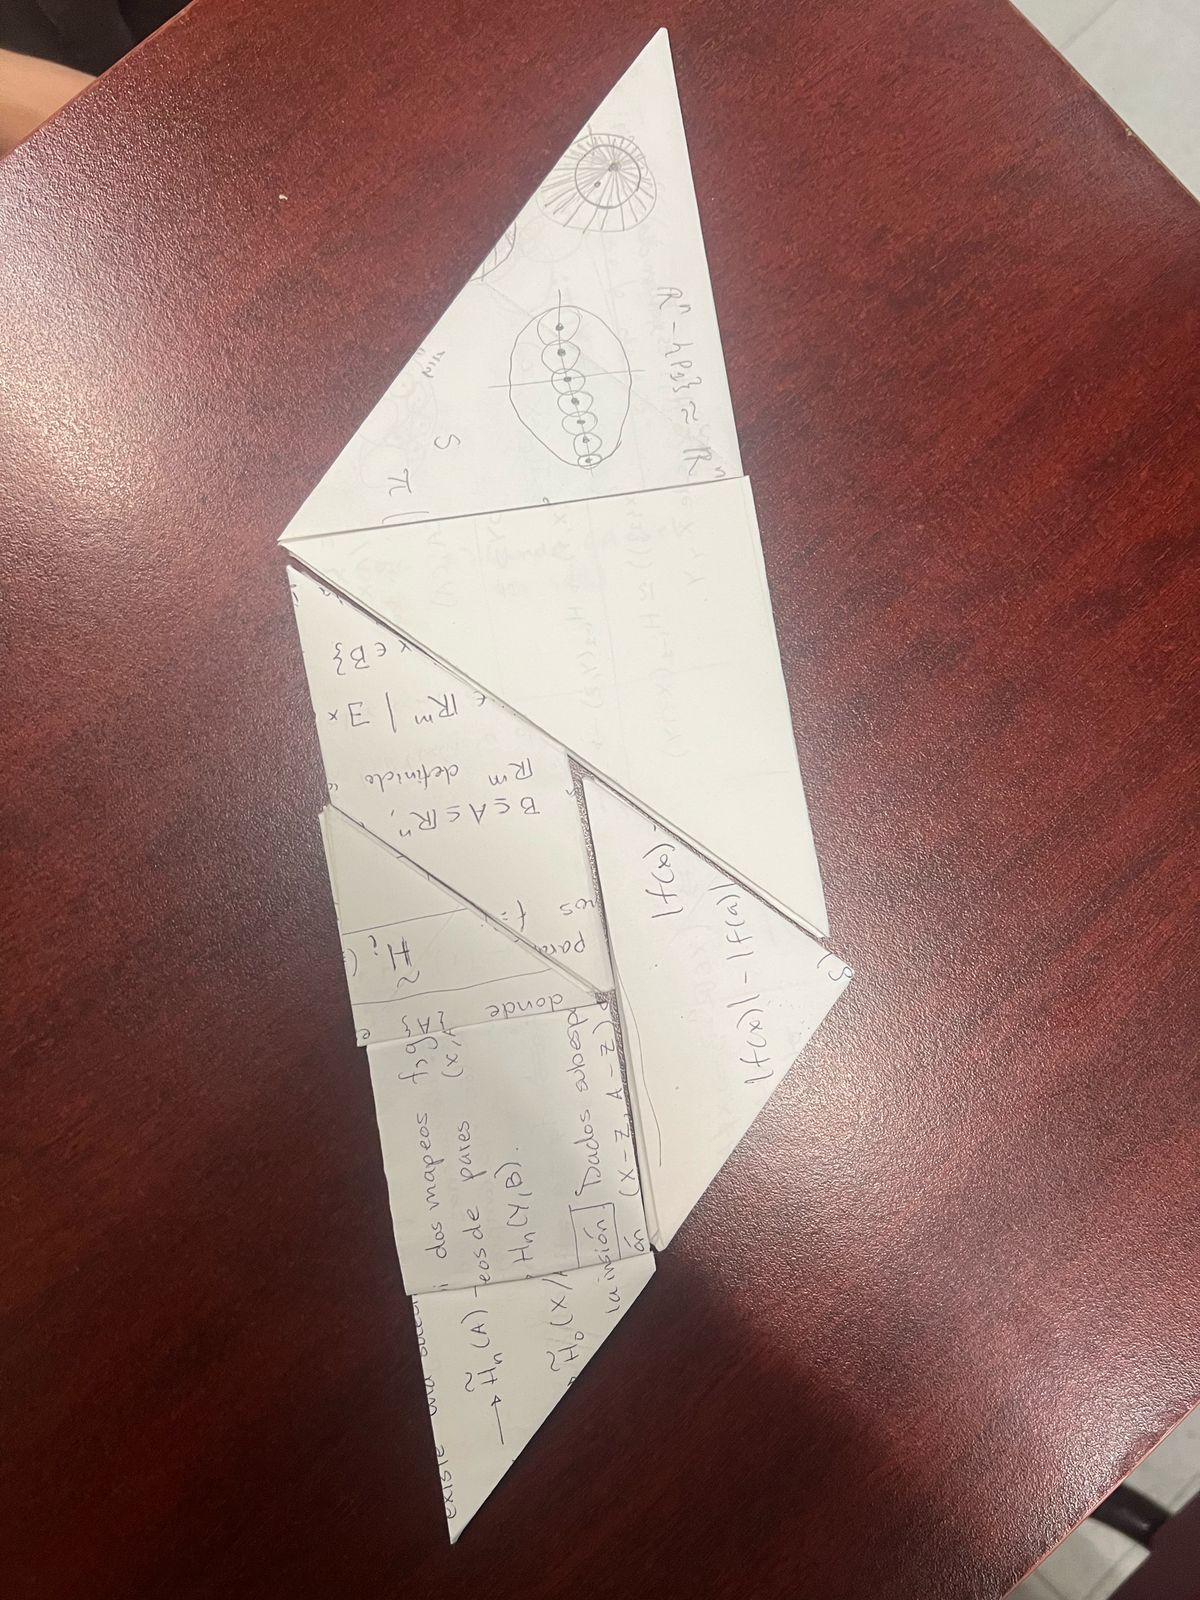
\includegraphics[scale=0.05]{clase2/rombo.jpeg} \\ \hline
    
            \end{tabular}        
    }

La forma en que realizamos cada figura fue comenzando con el cuadrado, a partir de él, buscando mover la menor cantidad de piezas para poder construir el resto de figuras, recordando que toda figura tienen una triangulación.
    
\end{itemize}